\documentclass[a4paper,11pt]{article}%
    
\usepackage{fullpage}%
\usepackage[T1]{fontenc}%
\usepackage[utf8]{inputenc}%
\usepackage[main=francais,english]{babel}% % Adjust the main language

\usepackage{graphicx}%
\usepackage{url}%
\usepackage{abstract}%

\usepackage{mathpazo}%

\usepackage{listings}%

\usepackage{subcaption}

\parskip=0.5\baselineskip

\sloppy

\begin{document}

\title{Activités, problèmes, résultats}

\author{Clément Legrand-Lixon}

\date{}

\maketitle

\paragraph*{22 Mai 2018}

Arrivée dans le laboratoire (Cristal). Rencontre de l'équipe (doctorants et stagiaires). Installation du poste de travail (Ubuntu, espace de travail : VSC, latex, R). Découverte du problème, recherche d'informations (variantes: multi-dépôts, avec capacité, avec limite de temps...). Lecture des articles \emph{A new enhancement of the Clarke and Wright savings heuristic for the capacitated vehicle routing problem} (K. Altınel, T. Oncan), et \emph{A simple, deterministic, and efficient knowledge-driven heuristic
for the vehicle routing problem} (Florian Arnold, Kenneth Sorensen). Vu administration pour la gratification de stage. 

\paragraph*{23 Mai 2018}

Fin de lecture des articles, résumé des articles tapés en tex. Implémentation de l'algorithme de Clarke and Wright (C W), en python.
Mise en place d'une heuristique basique (avec paramètre $\lambda$). 
Tests de l'algo sur des instances fabriquées aléatoirement. 
Tentative pour trouver une valeur optimale pour le paramètre selon la taille de l'entrée. 
Résultats disponibles avec la figure \ref{lambda}.

\begin{figure}[ht]
	\centering
	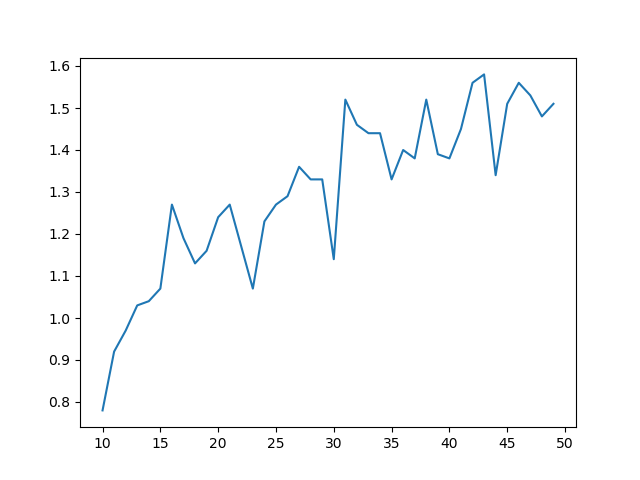
\includegraphics[width=0.7\textwidth]{best_lambda.png}
	\caption{Valeur de lambda optimale}
	\label{lambda}
\end{figure}

\paragraph*{24 Mai 2018}

Rencontre avec encadrante senior : Marie-Éléonore, bilan sur les premiers jours. Obtention du code C++ de l'heuristique de CW (complète, mais quelques erreurs présentes à corriger). 
\underline{Objectif}: Pour la semaine prochaine, faire une présentation reprenant la nouvelle heuristique développée dans l'article de F. Arnold et K. Sorensen. 
Et éventuellement implémentation des opérateurs locaux utilisés dans l'heuristique en expliquant les intérêts et limites de chaque (complexité, avantage...).  
Début de la présentation. Recherche d'articles détaillant les opérateurs utilisés. Peu de résultats (page wikipédia pour Lin Kernighan). 

\paragraph*{25 Mai 2018}

Rencontre avec Lætitia Jourdan (responsable de l'équipe). Implémentation de l'heuristique de Lin-Kernighan : pour une tournée donnée, optimise la visite des clients (utilisée pour TSP). Commence par réaliser 2-opt (cherche un changement entre deux arêtes qui améliore la tournée). Si trouvé on passe 3-opt (echange de 3 aretes), jusqu'à k-opt (k choisi). Puis applique la meilleure modif (la meilleure i-opt). S'arête lorsque plus d'améliorations possibles). 

Implémentation de 2-opt en python, tests sur quelques instances. On part de \ref{test1}, et en appliquant 2-opt on obtient \ref{test1_2opt}. 'Dépôt représenté en bleu). 

\begin{figure}[ht]
	\centering
	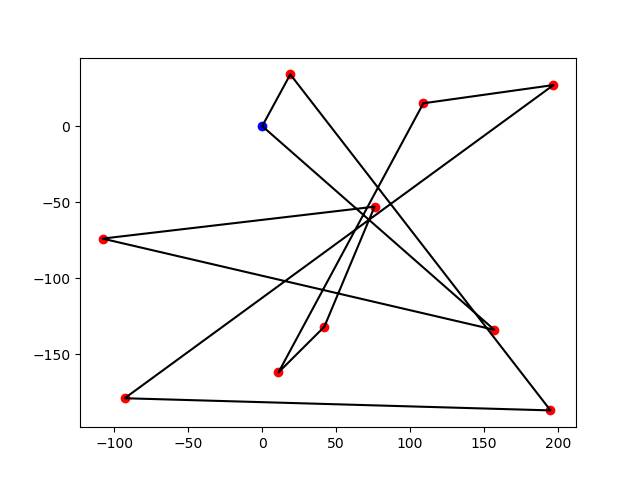
\includegraphics[width=0.5\textwidth]{test1_init.png}
	\caption{Instance initiale}
	\label{test1}
\end{figure}

\begin{figure}[ht]
	\centering
	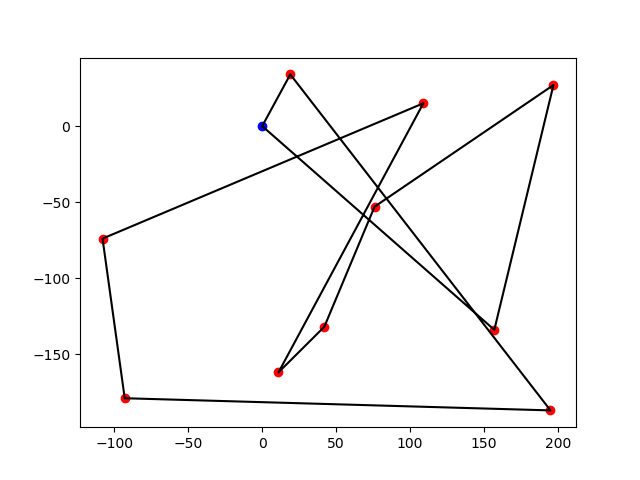
\includegraphics[width=0.5\textwidth]{test1_2opt.png}
	\caption{Optimisation avec 2-opt}
	\label{test1_2opt}
\end{figure}

Rencontre de problèmes avec des instances supérieures, et LK. $\rightarrow$ A résoudre lundi. Opérateur à utiliser principalement sur des petites portions de route, complexité élevée $O(n^k)$ avec $n$ le nombre de clients. 

\paragraph*{28 Mai 2018}

\underline{Objectifs} : finir d'implémenter LK, tester, et finir le développement dans la présentation. Améliorer présentation. Implémenter un autre opérateur \emph{Cross-exchange} ou \emph{Ejection-chain}.

\underline{Réalisation} :  LK corrigé (fonctionne avec 2-opt... généraliser à k-opt ?). Tests réalisés sur la tournée en image \ref{test4_20_init}, où on obtient la tournée en image \ref{test4_20_LKopt}.

\begin{figure}[ht]
\centering
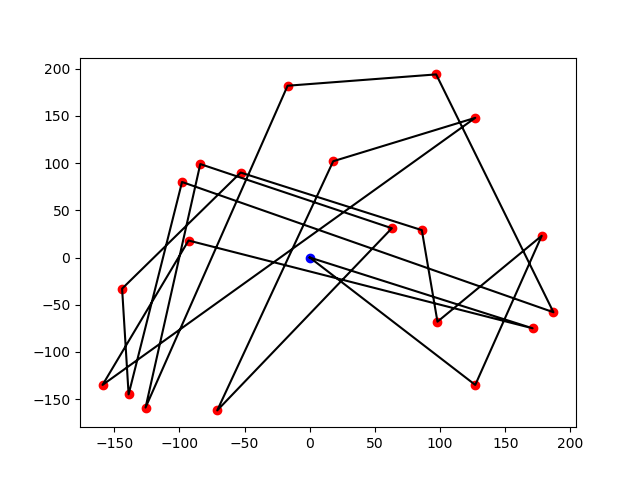
\includegraphics[width=0.5\textwidth]{test4_20_init.png}
	\caption{Instance initiale pour $20$ clients}
	\label{test4_20_init}
\end{figure}

\begin{figure}[ht]
\centering
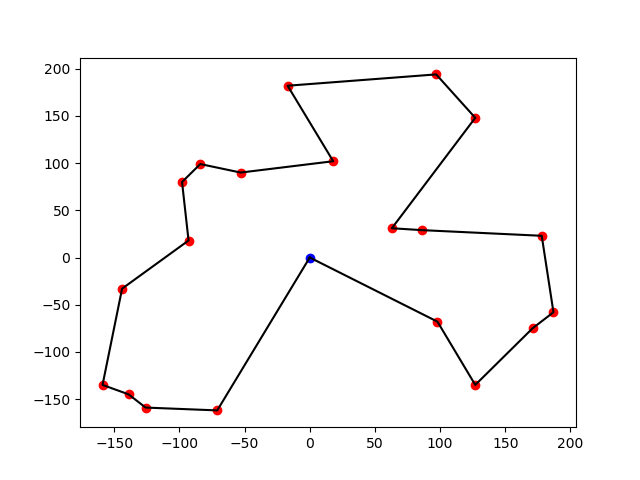
\includegraphics[width=0.5\textwidth]{test4_20_LKopt.png}
	\caption{Solution obtenue avec Lin-Kernighan}	\label{test4_20_LKopt}
\end{figure}

Début implémentation de Cross-exchange (local). Article détaillant cet opérateur : \emph{A Tabu Search Heuristic for the Vehicle Routing Problem with Soft Time Windows}. Cet opérateur consiste en l'échange de toute séquence de clients entre 2 tournées. L'aspect local est d'autant plus intéressant, que la complexité passe en quadratique dans le pire cas, au lieu de $O(n^4)$. 
On commence par calculer $k$ pp voisins pour chaque nœud (pré-calcul). Après avoir choisi une arête $(a,b)$, on regarde les plus proches voisins du premier nœud, on prend le premier qui est sur une tournée différente, $(c,v_a)$. 
On construit les deux arêtes $(a,v_a)$ et $(c,b)$. Puis on essaye d'échanger $(v_a+1, v_a+2)$, avec $(b+1,b+2)$, ou $(b+2,b+3)$ ainsi de suite jusqu'à retomber sur l'arête de départ ou trouver une amélioration. 
En pratique on trouve rapidement une amélioration d'où une complexité en général linéaire. 
Il faut aussi veiller à ne pas dépasser les contraintes de capacité (non prises en compte dans un premier temps). 
Fin implémentation, tests réalisés sur une instance particulière (cf ...), 3 exécutions ont été réalisées sur des arêtes différentes, (arête choisie en rouge). 
\end{document}